\section{Arhitektura dubokih mreža}
Duboke neuronske mreže pronašle su svoju primjenu u rješavanju mnogih zadataka strojnog učenja kao što su klasifikacija slika, analiza teksta, predviđanje vremenskih serija i sl. Pokazalo se nužnim, međutim, razviti nove slojeve neuronskih mreža da bi se ugradile pretpostavke prilagođene trenutnom zadatku. U ovom odjeljku predstavit ćemo slojeve koji se uobičajeno koriste u generatoru i diskriminatoru generativnih suparničkih mreža te aktivacijske funkcije primijenjene na njihove izlaze.

\subsection{Potpuno povezani sloj}
Potpuno povezani sloj je najjednostavniji sloj u neuronskoj mreži, a predstavlja afinu transformaciju ulaza u izlaz, tj. izlaz svakog neurona predstavlja linearnu kombinaciju ulaza kojoj je pribrojen neki konstantni faktor. Matrično, ovo možemo zapisati kao:
\begin{equation}
\vec{h} = W\vec{x} + \vec{b}
\end{equation}
gdje je $W$ matrica težina za svaki neuron, a $\vec{b}$ vektor pomaka koje pribraja. Tako je dimenzionalnost matrice $W$ $H \times N$, gdje je $N$ broj elemenata vektora na ulazu, a $H$ broj neurona u sloju. Naravno, $\vec{b}$ je $H$-elementni vektor jer je izlaz operacije $W\vec{x}$ istog broja elemenata.

Uobičajeno se koristi kao zadnji sloj u diskriminatoru da mapira izlaze prethodnih slojeva na skalarni izlaz, ili kao prvi sloj u generatoru da transformira ulazni slučajni vektor $\vec{z}$ u izlaz koji je uglavnom veće dimenzionalnosti. Neki autori \citep{karras2019style} u ovu svrhu koriste i više naslaganih potpuno povezanih slojeva uz manju modifikaciju o kojoj će više riječi biti kasnije.

\subsection{Konvolucijski sloj} 
Osnovna je zadaća konvolucijskoga sloja procesuiranje ulaza za koji znamo da je rešetkaste strukture \citep{Goodfellow-et-al-2016}, kao što su slike. Ime su dobile po tome što se umjesto operacije matričnog množenja, pri određivanju izlaza, koriste diskretnom konvolucijom matrice težina, čija je oznaka $*$. Dakle, određivanje izlaza konvolucijskog sloja možemo zapisati kao:
\begin{equation}
H = W * X + B
\end{equation}
Budući da su nam ulazi, u kontekstu generativnih suparničkih modela, slike, $X$ jest tenzor trećeg reda (visina, širina i broj kanala slike), kao i $H$ te $B$, dok je matrica težina $W$ tenzor četvrtoga reda (broj ulaznih kanala, broj izlaznih kanala, širina i visina prozora). $W$ u kontekstu konvolucijskoga sloja još nazivamo jezgrom, a $H$ mapom značajki. 
Izraz za diskretnu konvoluciju glasi:
\begin{equation}
(K * I)(i, j) = \sum_m\sum_nI(i - m, j - n)K(m, n)
\end{equation}
Primijetimo da je ovaj izraz prilagođen slučaju gdje su $K$ i $I$ tenzori drugoga reda. Međutim, vrlo lako možemo proširiti ovu definiciju kratkom analogijom s potpuno povezanim slojem. Kod potpuno povezanoga sloja, možemo primijetiti da težina $w_{ij}$ povezuje $i$-ti ulaz s izlazom $j$-toga neurona. U konvolucijskom sloju, tenzori su dimenzija $H_1 \times W_1 \times C_1$ i $H_2 \times W_2 \times C_2$, a već smo "osigurali" povezanost između visina $H_1, H_2$ i širina $W_1, W_2$. Ostaje nam još povezati mape značajki kojih ima $C_1$ u ulazu i $C_2$ na izlazu - u tu svrhu jednostavno alociramo konvolucijske jezgre za svako mapiranje (dakle, ima ih $C_1 \times C_2$). Formalno, $r$-ta mapa značajki određuje se kao:
\begin{equation}
H^{(r)} = \sum_s X^{(s)} * W^{(r, s)}
\end{equation}

Intuitivno, jezgre možemo zamisliti kao "prozore" određenih dimenzija kojima klizimo preko ulazne "slike" te izlazna vrijednost te operacije ovisi samo o vrijednostima koje su vidljive unutar prozora, čime konvolucija modelira efektivno modelira samo lokalne interakcije. Slika \ref{conv} vizualizira ovu ideju. Parametri prozora nisu ovisni o njegovoj poziciji, nego ostaju konstanti tijekom prijelaza. Time značajno smanjuje broj potrebnih parametara i omogućuje ekvivarijantnost na pomak. Funkcija $f$ je ekvivarijantna s obzirom na $g$ ako vrijedi $f \circ g = g \circ f$. U slučaju konvolucije, ako pomaknemo ulaz, pomaknut će se i mapa značajki, što je povoljno svojstvo kod obrade slika.

\begin{figure}[h]
\centering
		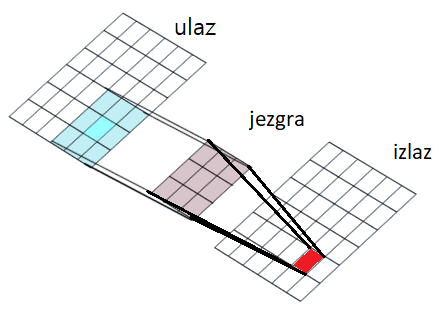
\includegraphics[width=0.8\textwidth]{images/conv.png}
\caption{Vizualizacija konvolucije.}
\label{conv}
\end{figure}

Kod uporabe konvolucijskog sloja, postoji nekoliko odluka koje korisnik mora donijeti između kojih je odabir pomaka prozora (ne mora se nužno prozor pomicati za samo jedan piksel), smanjivanje dimenzionalnosti izlaznog tenzora i broj izlaznih mapa značajki. Osvrnimo se kratko na problem smanjivanja dimenzionalnosti. Pretpostavimo da je ulazna slika dimenzija $H \times W$ (mape značajki u ovom trenutku nisu važne). Primijenimo li konvoluciju s jezgrom dimenzije $K \times K$, izlaz će biti $H - K +  1 \times W - K + 1$, a ne $H \times W$. To je ponekad poželjna funkcionalnost, ali češće bismo željeli da dimenzije slike ne opadaju s veličinom jezgre jer se konvolucijski slojevi često koriste slijedom jedan iza drugoga. Standardno je rješenje dodati $\left \lfloor \frac{k}{2} \right \rfloor$ nula sa svih strana ulaza čime izlaz postaje željenih dimenzija.

Može se pokazati da je gradijent konvolucije ponovno konvolucija, ovaj put gradijenata funkcije gubitka po izlazu sa jezgrom zrcaljenom oko središnjeg elementa. Ovu operaciju nazivamo transponiranom konvolucijom. Moguće ju je, također, koristiti u nekim slučajevima i u unaprijednom prolazu.

U kontekstu generativnih suparničkih mreža, konvolucija i transponirana konvolucija koriste se i u diskriminatoru i u generatoru. U diskriminatoru, koriste se kao osnovni dijelovi blokova kojim se smanjuje rezolucija ulaza - obavimo konvoluciju, rezultat propustimo kroz sloj sažimanja (o kojima ćemo nešto više reći kasnije) koji smanjuje dimenzionalnost izlaza konvolucije. Zatim novodobivene vrijednosti predamo kao ulaz idućem konvolucijskom sloju i to ponavljamo dok ulaz ne smanjimo do zadovoljavajuće veličine. 

S druge strane, u generatoru ponekad koristimo transponiranu konvoluciju s korakom većim od 1 - ovo efektivno omogućuje povećanje rezolucije slike s kojom radimo. Naime, uobičajeni pristup je generirati na početku tenzor male rezolucije (npr. $2 \times 2$) te transponiranom konvolucijom udvostručiti rezoluciju (tako da je jedan korak 2 piksela), gdje se nadamo da ćemo time popuniti nastale "rupe" dobivene širenjem tenzora nekom smislenom vrijednosti. 

Spomenimo još da, ako koristimo konvolucijski sloj gdje je korak samo 1 element, nije bitno jesmo li odabrali transponiranu ili "običnu" konvoluciju - jezgre će biti samo zrcaljene varijante jedna druge. 

\pagebreak
\subsection{Slojevi sažimanja i proširivanja}
Funkcija slojeva sažimanja i naduzorkovanja jest mijenjanje rezolucije ulaznog tenzora. Sloj sažimanja često se koristi u tandemu s konvolucijom u diskriminatoru da bi se povećalo receptivno polje značajki dubljeg sloja. Receptivno polje jest skup svih elemenata ulaznog sloja koje mogu utjecati na vrijednost te značajku. Pojasnimo na jednostavnom primjeru zašto je povećanje receptivnog polja povoljno za klasifikaciju u konvolucijskim modelima.

Pretpostavimo da naša ulazna slika prikazuje ljudsko lice. Prva konvolucija detektirala bi detalje niže razine, kao što je jedno oko, nos ili uho. Nakon što izlaz propustimo kroz sloj sažimanja, idućoj konvoluciji omogućavamo pogled na veći dio slike: tako možda uspije detektirati da ljudsko lice ima dva oka, dva uha i jedan nos. Apstrahiramo li ovaj primjer, možemo reći da sloj sažimanja omogućuje dubljim konvolucijskim slojevima modelirati značajke više razine.

Sažimanje se obično provodi određivanjem statističkih pokazatelja ulazne slike unutar nekog prozora, primjerice maksimalne ili prosječne vrijednosti. Problem smanjivanja širine i visine ulaznog tenzora koji se pojavljuje kod konvolucije prisutan je i kod sažimanja te je potrebno donijeti odluku hoćemo li nadopunjavati \engl{padding} ulaz nulama ili ne.

S druge strane, slojevi proširivanja u generatoru služe kao alternativa transponiranoj konvoluciji za povećavanje rezolucije. Naime, uporaba transponirane konvolucije često rezultira tvorevinama koje podsjećaju na šahovnicu (slika \ref{checkerboard}) \citep{odena2016deconvolution}. 

\begin{figure}[h]
\centering
		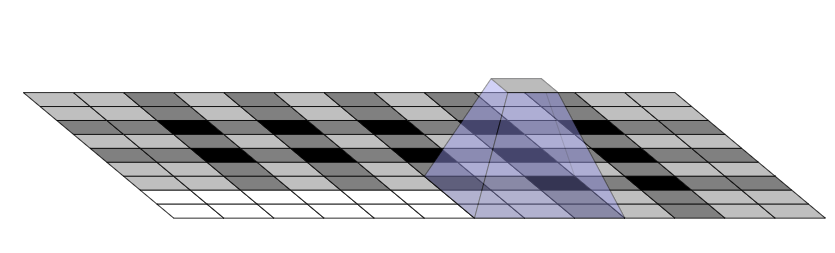
\includegraphics[width=0.8\textwidth]{images/checkers_reason.png}
\caption{Vizualizacija uzroka šahovskog uzorka. Konvoluciju s jezgrom $3 \times 3$ provodimo uz korak duljine 2. Što je element tamniji, više je elemenata uključeno u njegov izračun. Preuzeto iz \cite{odena2016deconvolution}}
\label{checkers_reason}
\end{figure}
		
\begin{figure}[h]
\centering
		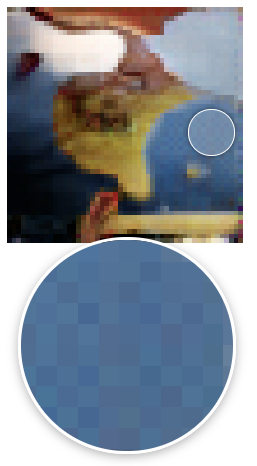
\includegraphics[height=0.5\textwidth]{images/checkers.png}
\caption{Primjer tvorevina koje podsjećaju na šahovnicu. \cite{dumoulin2016adversarially}, preuzeto s https://distill.pub/2016/deconv-checkerboard/}
\label{checkerboard}
\end{figure}

Uzrok ovome je što u nekim slučajevima određenim elementima tenzoru više rezolucije pridonosi više elemenata niže rezolucije nego ostalima (slika \ref{checkers_reason}). 

Da bi se izbjegla ova pojava, istraživači su se okrenuli kombinaciji proširivanja ulaznog tenzora i konvoluciji s jediničnim korakom (i nadopunjavanjem). Postoji nekoliko načina proširivanja, ali najčešće se, zbog jednostavnosti, koristi proširivanje uz interpolaciju pomoću najbližeg susjeda: vrijednost nepoznatih piksela povećane slike određuje se kao vrijednost najbližeg poznatog piksela. Na rezultirajući tenzor zatim primijenimo konvoluciju da bismo prilagodili vrijednosti novih piksela na finiju rezoluciju.  